%!TEX root = Main.tex
\documentclass[Main]{subfiles}

\begin{document}

\section{Software} % (fold)
\label{sec:software}

	In this project, software was a vital part. 
	While the course theory had presented ways of doing 
	In this chapter, the coding environment, structure and behaviour of the codebase will be covered.
	
	\subsection{Environment} % (fold)
	\label{sub:software_environment}

<<<<<<< HEAD

		The software for this project was written in C++ using the Xilinx Software Development Kit.
		C++ was chosen because it is a object oriented library, which gave some clear advantages when working in a three person team.
		Furthermore, C++ has native support for an resizable array datatype known as a vector, which greatly reduced the complexity of manipulating array.
		The software was written for the C++11 standard, since the standard gave some advantages in initialisation of vectors.
		GitHub was used for version control	to manage and backup code.
		
		\fxnote{Write Something about Map}
		
		\subsection{Design} % (fold)
		\label{sub:software_design}

>>>>>>> origin/master
	
	\subsubsection{Structure} % (fold)
	\label{subsub:software_structure}
		A object-oriented approach was taken to the design, in order to modulize the different parts of the software. 
		
		This gave clear advantages when working multiple people on the same codebase, as the development of the different classes could be spread out between multiple people.
		
		The structure of the software is depicted in \autoref{fig:classdiagram} as a UML class diagram.
		
		\begin{figure}[H]
			\centering
			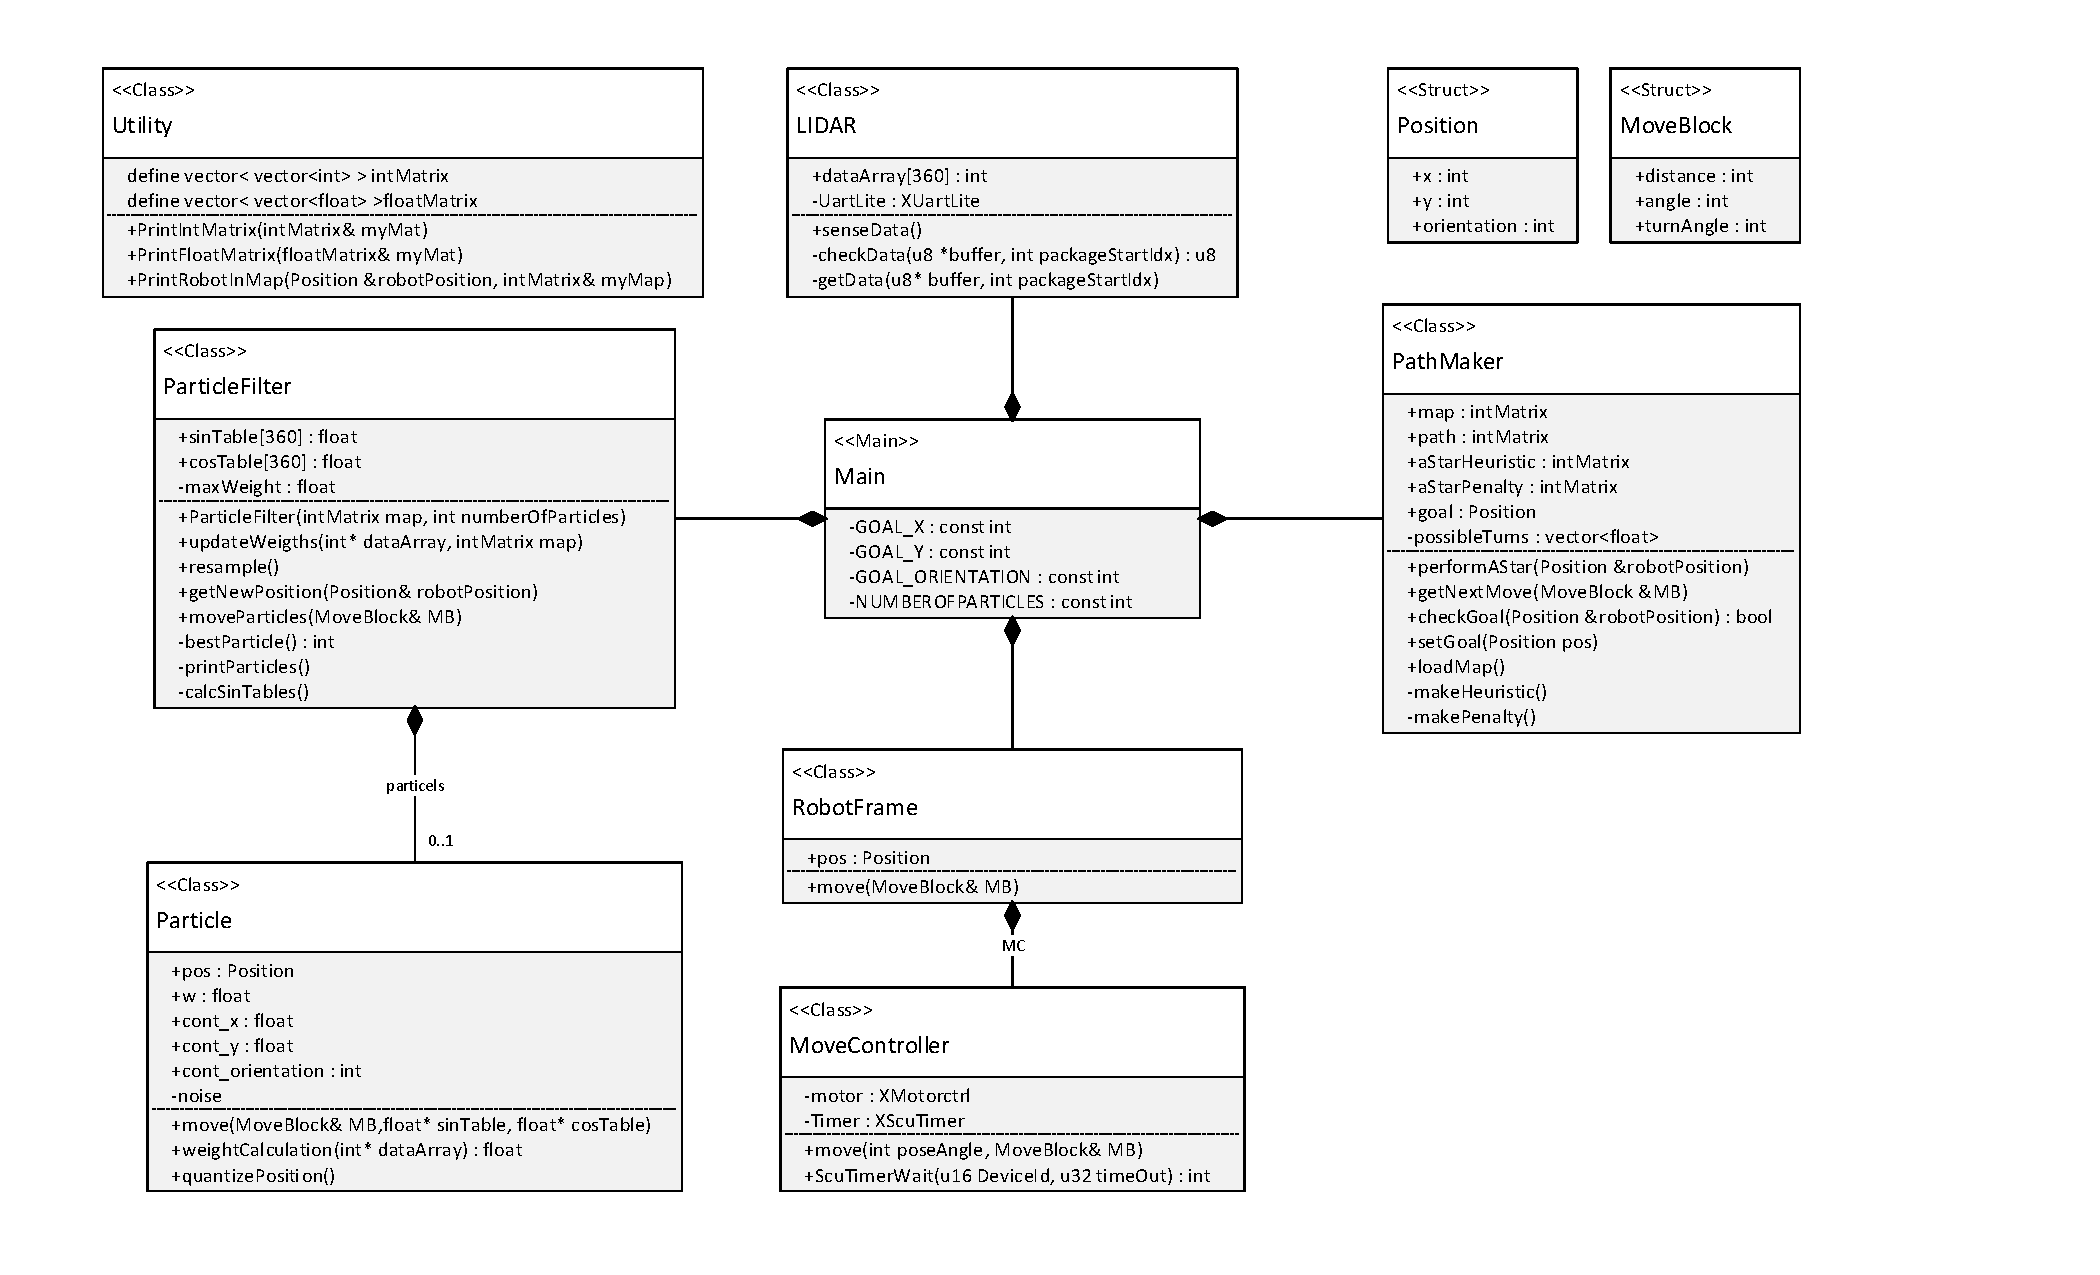
\includegraphics[width=\linewidth]{ClassDiagram}
			\caption{Class Diagram}
			\label{fig:classdiagram}
		\end{figure}

<<<<<<< HEAD

		The main components of the program is the LIDAR, PathMaker, RobotFrame and ParticleFilter classes. 
		Each class has a distinct purpose, which maps directly to one of the four  actions in the main loop of \autoref{fig:systemact}.
		The mapping can be see in \autoref{table:action_class_map}
		 
		\begin{table}[H]
			\centering
			\begin{tabular}{|c|c|}
			\hline
				Action & Class \\ 
			\hline
				A2: Sense Data & LIDAR  \\ 
			\hline
				A3: Estimate Robot Position & ParticleFilter  \\ 
			\hline
				A4: Calculate Path & PathMaker  \\ 
			\hline
				A5: Move & RobotFrame  \\ 
			\hline
			\end{tabular}
			\caption{Grid map for demonstration}
			\label{table:action_class_map} 
		\end{table} \noindent
>>>>>>> 26f5c724e65058c0cc90ada9450d0d0a17e7fbe5
		
<<<<<<< HEAD
	\subsubsection{Behaviour} % (fold)
	\label{subsub:software_behaviour}
>>>>>>> origin/master
	
		The dataflow between the different classes is covered in the Internal Block Diagram in \autoref{fig:softwareibd}
		
		\begin{figure}[H]
			\centering
			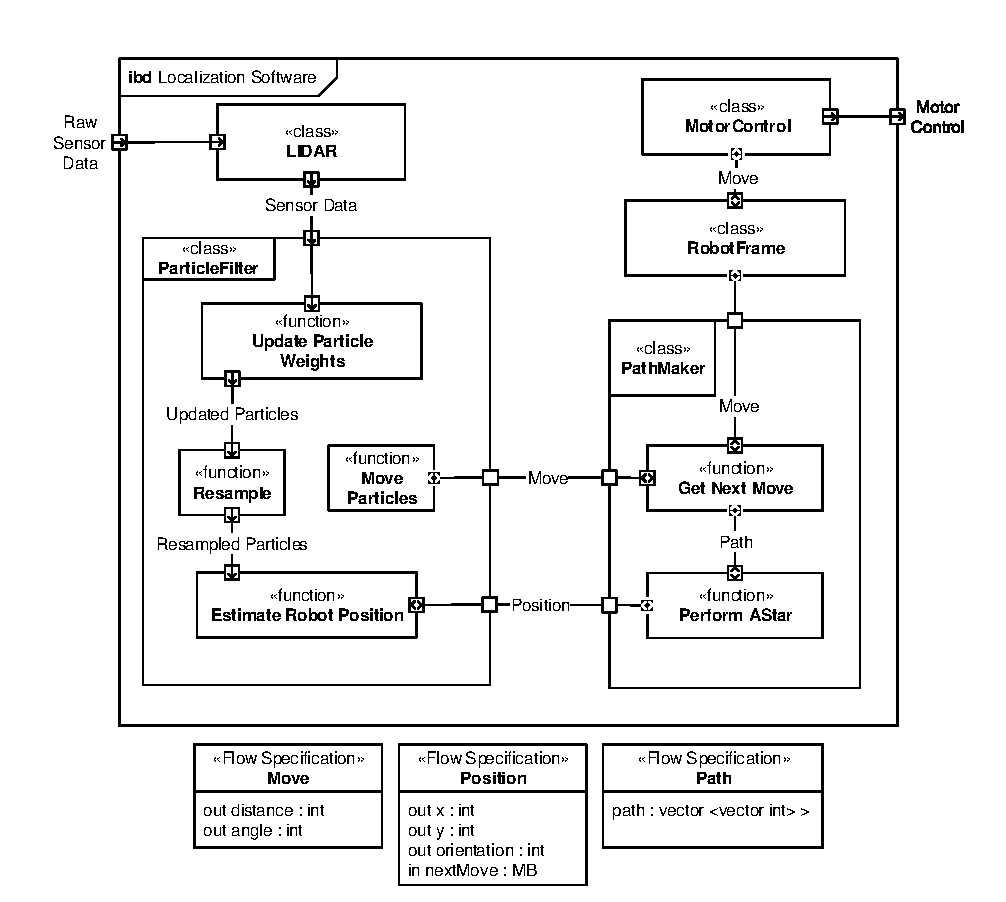
\includegraphics{SoftwareIBD}
			\caption{Software Internal Block Diagram}
			\label{fig:softwareibd}
		\end{figure}

		The raw sensor data from the Sensing block in \autoref{fig:systemibd} is sent to the LIDAR class, which  converts the raw sensor data to 360 distance values.
		The sensor data is sent to the ParticleFilter class, which update its current particle weights. 
		These weights are used to resample the particles using the low variance sampling technique presented in the course material.
		The robots position is then estimated by taking the position of the particle with the biggest weight.
		This position is used in the PathMaker, which performs AStar to find the best path to the goal. The next move from this path is then sent to both the RobotFrame class and the ParticleFilter, to move both the robot and the Particles along the expected path.
		The RobotFrame class uses the MotorControl class to send a control signal to the Motion block from \autoref{fig:systemibd}, which converts the control to a PMW signal that controls the motors of the robot.
<<<<<<< HEAD
	
	\subsection{Implementation} % (fold)
	\label{sub:software_implementation}
	
	The code was implemented according to the design. The code can be found in \fxnote{CodeBae Reference}.
	

		\begin{lstlisting}[caption=Example of CNN setup, style=Code-Matlab, label=lst:cnn_setup]

			% Insert code here

		\end{lstlisting}

>>>>>>> origin/master
% section software (end)
\end{document}